\documentclass[10pt,a4paper]{article}
\usepackage[utf8]{inputenc} % para poder usar tildes en archivos UTF-8
\usepackage[spanish]{babel} % para que comandos como \today den el resultado en castellano
\usepackage{a4wide} % márgenes un poco más anchos que lo usual
\usepackage[conEntregas]{caratula}
\usepackage{mathtools}
\usepackage{float}
\usepackage[pdftex]{graphicx}
\usepackage{caption}
\usepackage{subcaption}
%\usepackage{Sty/algorithm2e}
\usepackage[ruled,vlined]{algorithm2e}
%Esto de abajo es para encabezado y pie de pagina
\usepackage{lastpage}
\usepackage{fancyhdr}
\usepackage{amsfonts}
\usepackage{verbatim}
\usepackage{color}

%Esto es para configurar márgenes
\textheight=25cm
\textwidth=18cm
\topmargin=-1.5cm 
\oddsidemargin=-1cm 

\usepackage{wrapfig}
\usepackage{multirow} 

\pagestyle{fancy}
%\fancyhf{} % clear all header and footer fields
%\fancyfoot[R]{\footnotesize Página \thepage\ de \lastpage\}

\cfoot{\thepage /\pageref{LastPage} }

\newcommand\BlockIf[1]{\KwSty{If} \\ #1 \\ \KwSty{End If}}
\newcommand\BlockElseIf[1]{\KwSty{Else If} \\ #1 \\ \KwSty{End Else If}}
\newcommand\BlockElse[1]{\KwSty{Else} \\ #1 \\ \KwSty{End Else}}

\begin{document}

\titulo{Trabajo Práctico 2}
\subtitulo{Aprendizaje por Refuerzos}

\fecha{\today}

\materia{Aprendizaje Automático}
\grupo{}

% Pongan cuantos integrantes quieran
\integrante{Abdala, Leila Yasmin}{950/12}{abdalaleila@gmail.com}
\integrante{Bertero, Federico Alberto}{}{federico.bertero@gmail.com}
\integrante{Costa, Manuel José Joaquín}{035/14}{manucos94@gmail.com}


\maketitle

\newpage
\section{Modelo}
Para modelar el tablero se empleó una matriz de 6 filas por 7 columnas. En particular, se escogió la representación de vector de vectores columna por parecernos más natural para modelar el juego (en comparación a usar vectores fila).
Las fichas son representadas con los caracteres "R" para el caso de las fichas rojas, "Y" en el caso de las amarillas y finalmente usamos el carácter " " para indicar que el casillero se encuentra vacío.

Se utilizó el formalismo estándar definido en la materia para especificar el problema. El conjunto de estados se define como todos los tableros alcanzables agregando una ficha por cada turno de jugador. Por ejemplo, no se considera como un estado un tablero con solo dos fichas rojas, porque este tablero solo se podría obtener si el jugador rojo agregara dos fichas seguidas. Ademas, no se considera como un estado un tablero donde se agreguen más fichas de la capacidad de cada columna. Es decir, si tenemos una columna donde ya se han colocado seis fichas, se restringe la posibilidad de que se agregue una nueva ficha a dicha columna\footnote{Ver definición de conjunto de acciones.}. Cabe destacar que la cantidad de estados posibles, sin restringir el modo de agregar fichas, es $3^{6*7}$. Este tamaño implicaría que cualquier búsqueda dentro del espacio de estados no pueda realizarse de forma eficiente. Si bien por las restricciones del juego este espacio termina siendo sensiblemente menor (no es trivial precisar cuánto), no deja de tener un tamaño considerable.

El conjunto de acciones indica en que columna se podría agregar la ficha en el estado actual. Se definió la función $available\_moves:estado \rightarrow \{accion\}$, que dado un estado nos devuelve cuales son las acciones posibles que se podrían llevar a cabo en el mismo.

Dado un estado y una acción, la función de transición devuelve el estado resultante de ejecutar dicha acción por el jugador actual (es decir, el que poseía el turno). En este caso, la función de transición tomará un estado, representado por un tablero T con fichas, y una acción A, y devolverá el estado resultante de agregar en el tablero T una ficha en la columna indicada por la acción A. %probablemente habria que aclarar como se maneja el color de la ficha, no estoy segura

Finalmente se define la función de recompensa que otorga puntajes de: 1 al ganador, -1 al perdedor, y 0.5 a ambos si fue empate. En el caso particular del qlearner, esta es la función que desata el aprendizaje.

\subsection{Método de aprendizaje}

Para entrenar al agente se utilizó el algoritmo de Q-Learning. El motivo de esto es que Q-Learning al ser model-free, nos permite trabajar con un subconjunto de estados que definiremos a medida que se ejecuta el aprendizaje. Nótese que Q-Learning asume que el estado siguiente siempre depende del agente, lo que se usa al momento de realizar el aprendizaje. Sin embargo, dado que este juego es por turnos, nos es imposible determinar con certeza cual va a ser el siguiente estado. Para sortear este problema se implementó una solución en la que el jugador $R$ intenta adivinar el movimiento que va a realizar el contrincante $Y$. Para esto, $R$ se posiciona en el tablero como si fuera $Y$, es decir como si jugara con las fichas del otro color, y en base a su propia experiencias (su función Q) elige la acción A que maximizaría la recompensa de $Y$. Luego el jugador $R$ asume que $Y$ realizó la acción A y actualiza su Q.

Al inicio del aprendizaje se usa un $Q(s,a) = 1 \forall a,s$. Se utiliza la estrategia softmax para elegir las acciones en cada turno. En cada turno se actualiza el aprendizaje en Q(S,a), sin embargo, la función de recompensa solo asigna un puntaje distinto de cero en los estados terminales.

\newpage
\section{Experimentación}
Dedicamos la presente sección al estudio de diferentes hipótesis e incógnitas que se fueron planteando, y que influyen en la forma en que se lleva a cabo el aprendizaje. Se lista cada una de ellas como un item y se acompaña por una descripción del experimento asociado, junto a sus resultados.


\begin{itemize}
	\item ¿Cuándo decidimos cortar el aprendizaje?

	Se utilizó un número fijo de iteraciones (partidas donde el jugador aprende) que se obtuvo luego de ver como se comporta la función que describe el \emph{rate} de partidas ganadas por el jugador $R$ ($wins_R$ $\slash$ $partidas\_jugadas$), del tipo bot (QLearning), al jugar contra el jugador $Y$, del tipo random. 
	
	Como se puede ver en la figura~\ref{figura1}  y en el cuadro~\ref{tabla1}, la función converge al valor 0.76 y si bien es estrictamente creciente, a partir de la iteración 300.000, registra creces despreciables ($\simeq$0.005 en las 300.000 siguientes). Es por ello que definimos 300.000 como el numero de iteraciones a realizar (partidas a jugar) en la etapa de aprendizaje.
	
	Se podría utilizar, como alternativa, un criterio de parada del tipo, mientras en las ultimas $X$ iteraciones el ratio de partidas ganadas por 'Y' sea mayor a un determinado valor chico $\varepsilon$, continuar aprendizaje
	
	\begin{table}[H]
    \centering
	\begin{tabular}{c | c}
		Iteraciones & $win\_rate_R$ \\
		\hline
		\hline
       10000  & 0.661733826617 \\
       20000  & 0.699015049248 \\
       30000  &  0.713476217459 \\
       40000  &  0.724031899203 \\
       50000  &  0.730185396292 \\
       60000  &  0.733187780204 \\
	   70000  &  0.736489478722 \\
       80000  &  0.73814077324 \\
       90000  &  0.740369551449 \\
       100000  & 0.742222577774 \\
				& . \\
				& . \\
				& . \\
       \color{red}{300000 } & \color{red}{0.754387485375} \\
				& . \\
				& . \\
				& . \\
       600000  &  0.759312272352 
	\end{tabular}
	\caption{Tasa de victorias del bot a medida que avanzan las iteraciones.}
	\label{tabla1}
	\end{table}
	
	\begin{figure}
    	\centering
		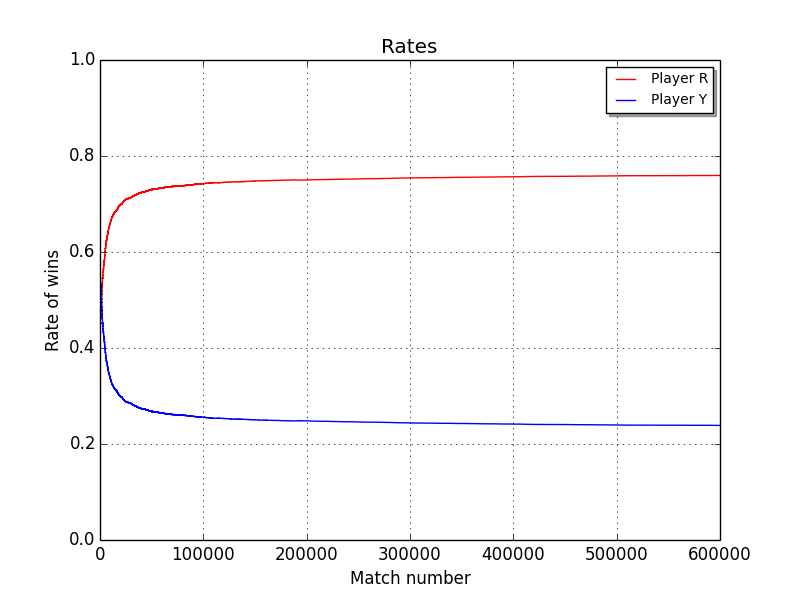
\includegraphics[scale=0.50]{graficos/iteracionespng.png}
		\caption{En rojo, la tasa de victorias del bot a medida que avanzan las iteraciones. En azul, la tasa de victorias del jugador random.}
		\label{figura1}
	\end{figure}
	
	\item ¿Cuales son los mejores valores que le podemos asignar a los parámetros $\alpha$, $\gamma$, $\tau$? 
	
	Para la elección de los valores asociados a los parámetros $\alpha$, $\gamma$ y $\tau$, se optó por ejecutar el aprendizaje sobre una lista de posibles valores para cada uno de ellos y tomar aquellos con los que se obtuvo el mejor resultado. Específicamente:
	
	\begin{itemize}
		\item $\alpha$ se itero sobre la lista $[0.1, 0.3, 1.0]$.
		\item $\gamma$ se itero sobre la lista $[0.8, 0.85, 0.9, 0.95]$.
		\item $\tau$ se itero sobre la lista $[0.05, 0.1, 0.5, 1.0]$.
	\end{itemize}
	
	En la figura~\ref{fig:grid} se pueden ver reflejados los resultados que se obtuvieron luego de ejecutar el grid-search como se describió anteriormente. Lo más interesante de dicha figura, a nuestro entender, es la clusterización que se produce, en tres grupos bien definidos. Dicho agrupamiento, puede verse, está dado exclusivamente por los valores de $\tau$. Es notable que entre más pequeño es el valor de este hiperparámetro, mejor se desempeña el agente. Esto nos dice que el sistema no favorece la exploración. Probablemente se deba a que el juego penaliza fuertemente los errores, lo que implica que jugar con un alto grado de azar no es buena idea pudiéndose hacer algo "mejor".
    
    Por otra parte, el resto de los parámetros no parecen tener una influencia demasiado fuerte sobre los resultados, aunque se ve una preferencia por $\alpha = 1$ en los primeros lugares. Por lo tanto, el agente se inclinará al máximo por aprender, le dará poca importancia a la información que ya tiene. 
    
    Sobre $\gamma$ podría haber sido más enriquecedor poner valores más chicos, aunque nos movimos bajo la convención estándar de que valores cercanos a $0.9$ suelen ser buenos, lo que además se condecía bien con nuestra hipótesis de que al momento de tomar una acción, el agente debería darle más importancia a las recompensas que puede obtener a partir de acciones lejanas, pues si el juego pudiera resolverse bien escogiendo siempre óptimos locales no sería desafiante para máquinas ni personas. 
		
	\begin{figure}
    	\centering
		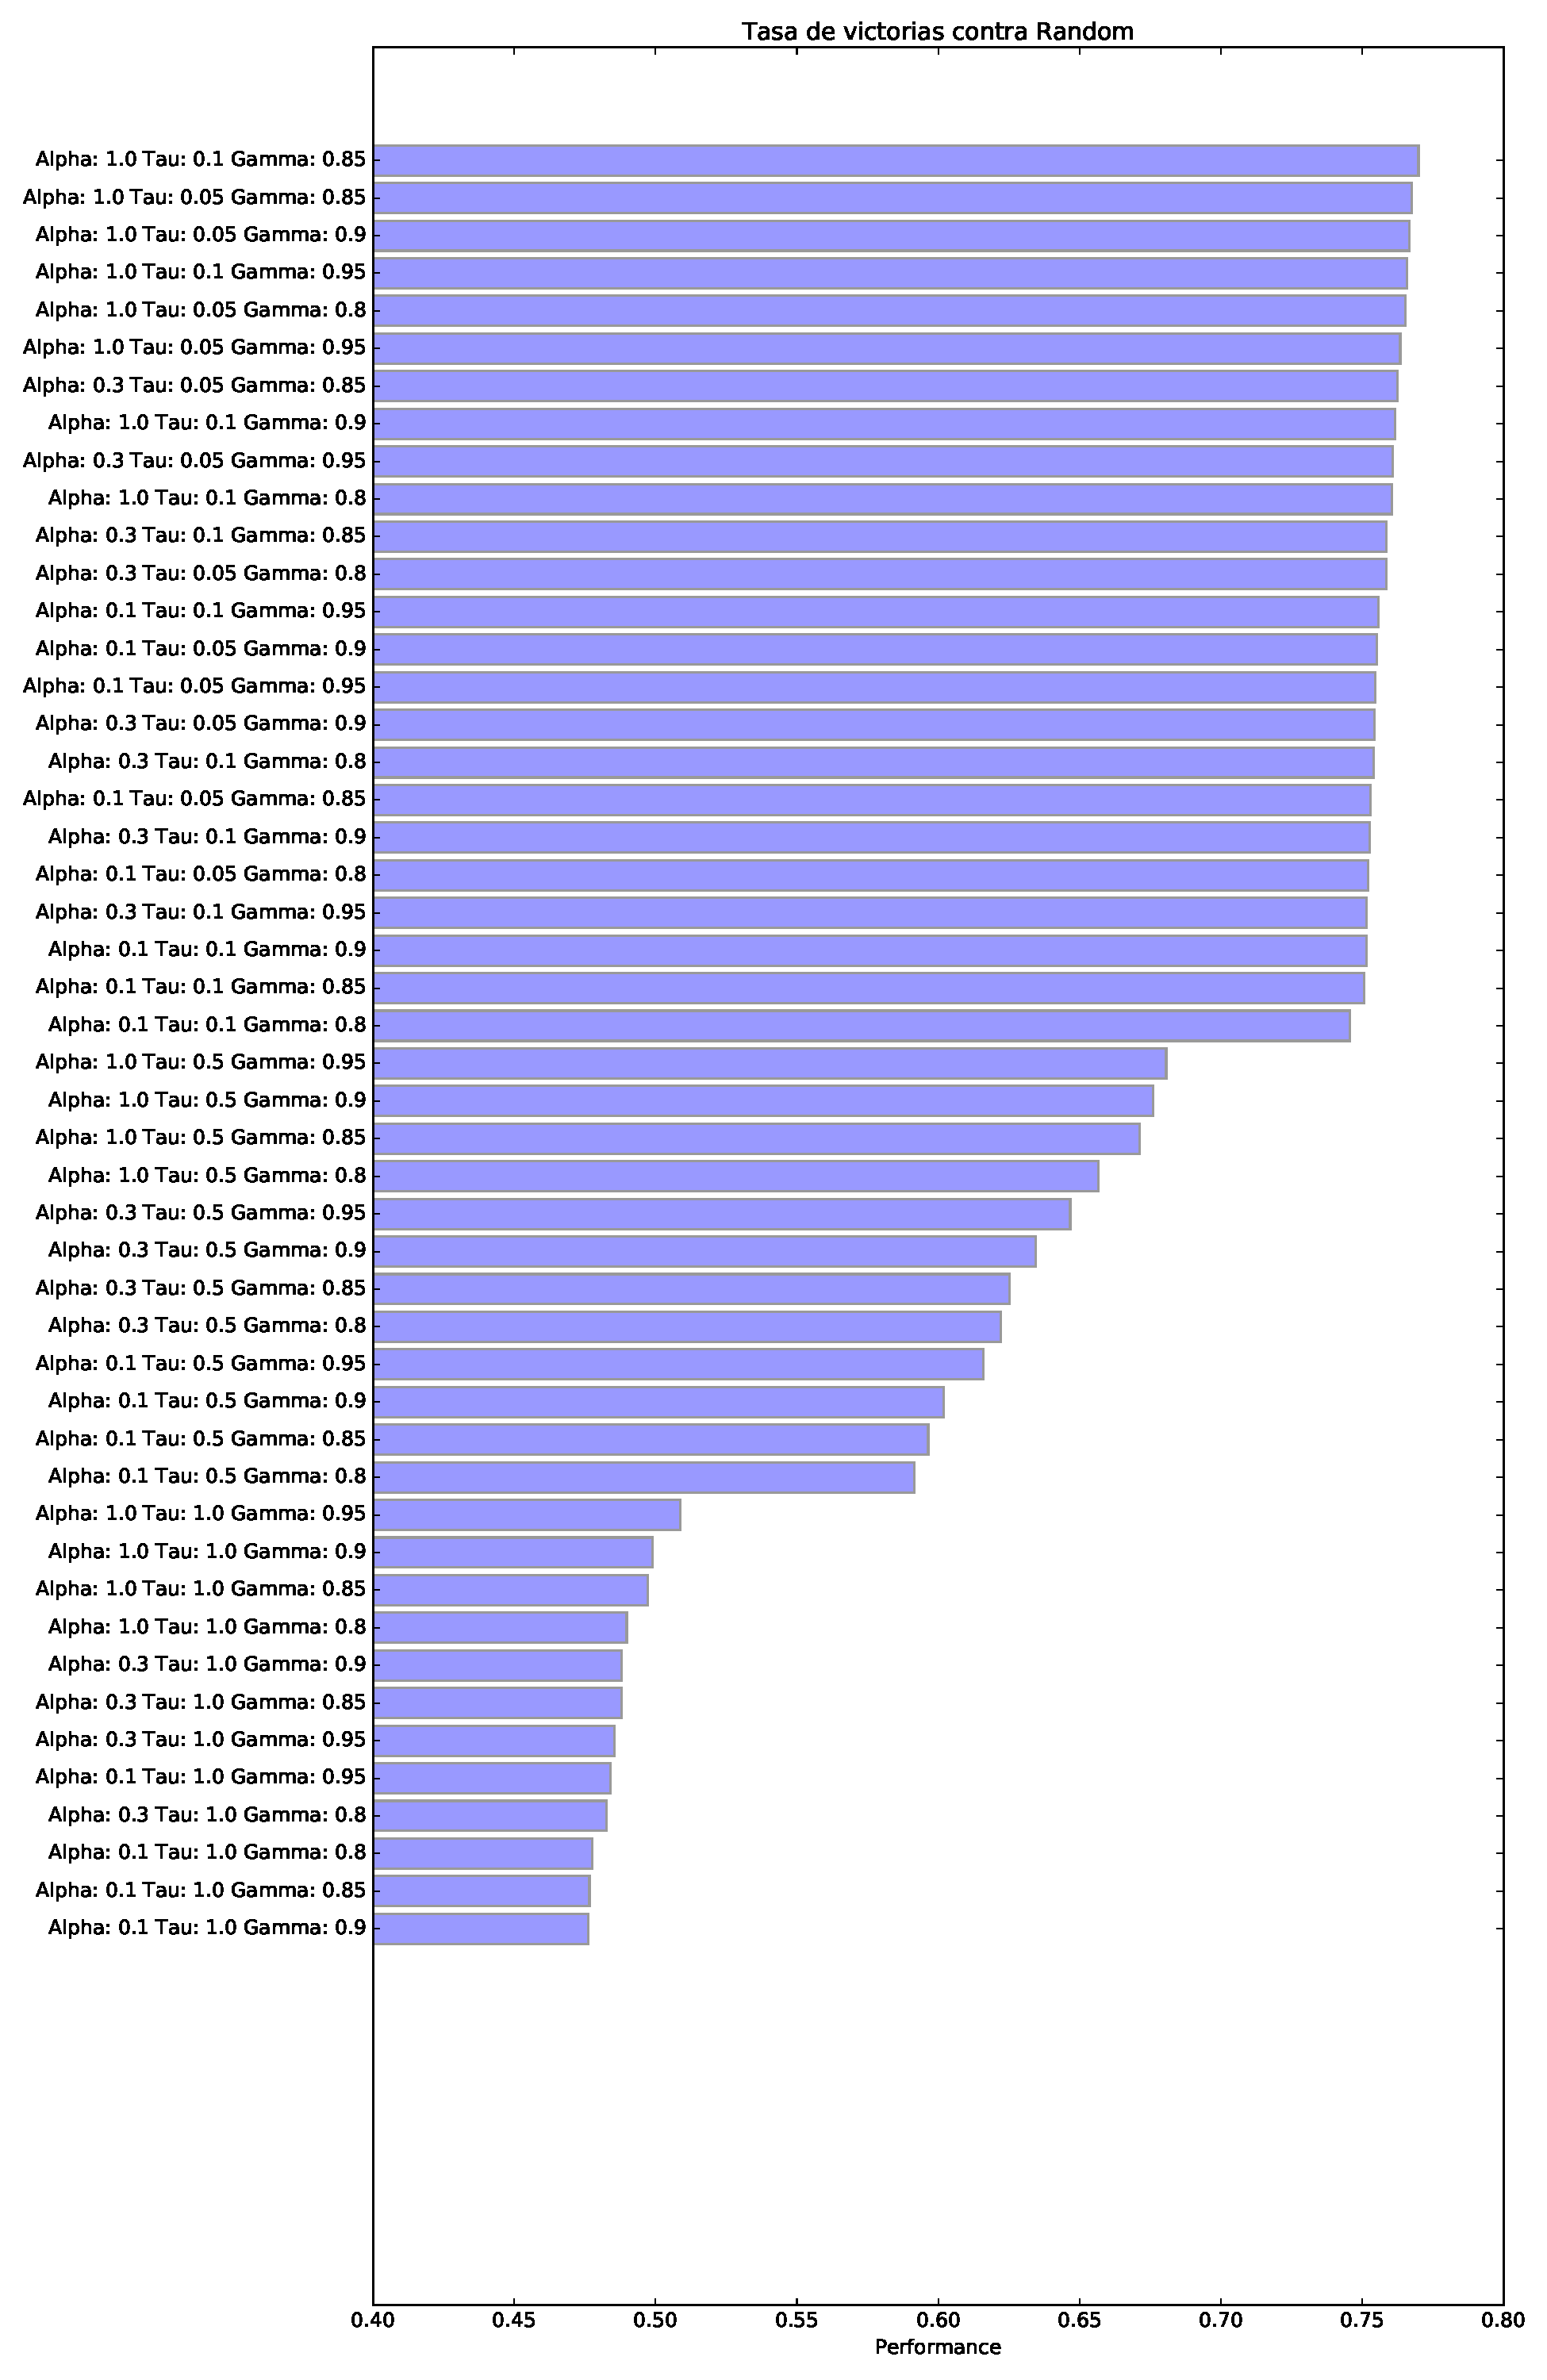
\includegraphics[scale=0.48]{graficos/grid_search.pdf}
		\caption{Resultados del \emph{grid search}. La performance se midió como el rate de victorias del qlearner sobre el último 10\% del total de las iteraciones (200k)}
		\label{fig:grid}	
	\end{figure}

		
\item ¿Cuánto influye en el aprendizaje el modo de jugar del oponente?

	Este experimento se divide en tres partes. En la primera se entrenó al jugador $R$, del tipo bot (QLearning), jugando contra el jugador $Y$, del tipo random, en 300000 iteraciones. La tasa parcial de aprendizaje se puede observar en la tabla 3. Luego se procedió a evaluar el beneficio de este aprendizaje compitiendo contra un nuevo jugador $X$, del tipo bot, sin entrenar. Para esto se itero 15000 veces, con ambos jugadores aprendiendo. La tasa de victorias para el jugador $R$ fue 0.48967, y para el jugador $X$ 0.500667.
    
	\begin{table}[H]
    \centering
	\begin{tabular}{c c}
       10000 iteraciones & Rate =  0.67613 \\
       20000 iteraciones & Rate =  0.74053\\
       30000 iteraciones &  Rate =  0.7506 \\
       40000 iteraciones &  Rate =  0.75667 \\
       50000 iteraciones &  Rate =  0.7622667 \\
       60000 iteraciones &  Rate =  0.7610667 \\
	     70000 iteraciones &  Rate =  0.7577333 \\
       80000 iteraciones &  Rate =  0.759667\\
       90000 iteraciones &  Rate =  0.767 \\
       100000 iteraciones & Rate =  0.7558 \\
				& . \\
				& . \\
				& . \\
       300000 iteraciones & Rate = 0.765466666667

	\end{tabular}
	\caption{}
	\end{table}

En base a estos resultados se observó que el aprendizaje contra el tipo random no aportaba positivamente al desempeño del jugador contra el tipo bot. Esto podría deberse a que la complejidad de decisión del tipo bot es mucho mayor que el tipo random, por lo que optamos por invertir este experimento para validar nuestra intuición.

En esta segunda parte se entreno al jugador $R$, del tipo bot (QLearning), al jugar contra el jugador $Y$, también del tipo bot, en 60000 iteraciones. La tasa parcial de aprendizaje se puede observar en la tabla 4. Luego se procedió a evaluar el beneficio de este aprendizaje compitiendo contra un nuevo jugador $X$, del tipo random. Para esto se itero 15000 veces, con ambos jugadores aprendiendo. La tasa de victorias para el jugador $R$ fue: 0.680266666667 y para el jugador $X$: 0.316733333333.

	\begin{table}[h]
    \centering
	\begin{tabular}{c c}
       15000 iteraciones & Rate =  0.4986 \\
       30000 iteraciones & Rate =  0.4906\\
       45000 iteraciones &  Rate =  0.4924667 \\
       60000 iteraciones &  Rate =  0.4912667 \\
	\end{tabular}
	\caption{}
	\end{table}

Luego de analizar estos resultados concluimos que el aprendizaje de nuestro agente es directamente dependiente del tipo de jugador con el que compite. De esta conclusión surge una nueva pregunta: ¿Cuánta ventaja obtiene realmente el jugador de tipo bot al entrenarse previamente, respecto a otro jugador de tipo bot que no ha aprendido nada?

Este pregunta tiene su foco en intentar deducir cuantas iteraciones son realmente necesarias en realidad para que un jugador "X" de tipo bot aprenda a jugar contra otro de tipo bot, pues se ha tomado como axioma que la tasa de victorias de ambos jugadores se estabiliza cuando ninguno puede aprender nuevas formas de vencer a su rival.

Para la tercer y última parte de nuestro experimento se entrenó al jugador $R$ contra otro jugador del tipo bot, en 100000 iteraciones. Luego se itero 10000 contra un nuevo jugador "Y" también de tipo bot, pero este sin entrenamiento previo. La figura 3 solo muestra la tasa de victorias de las primeras 1000 iteraciones, ya que a partir de la iteracion 800 no se observan cambios en el comportamiento.

\begin{figure}[H]
	\centering
		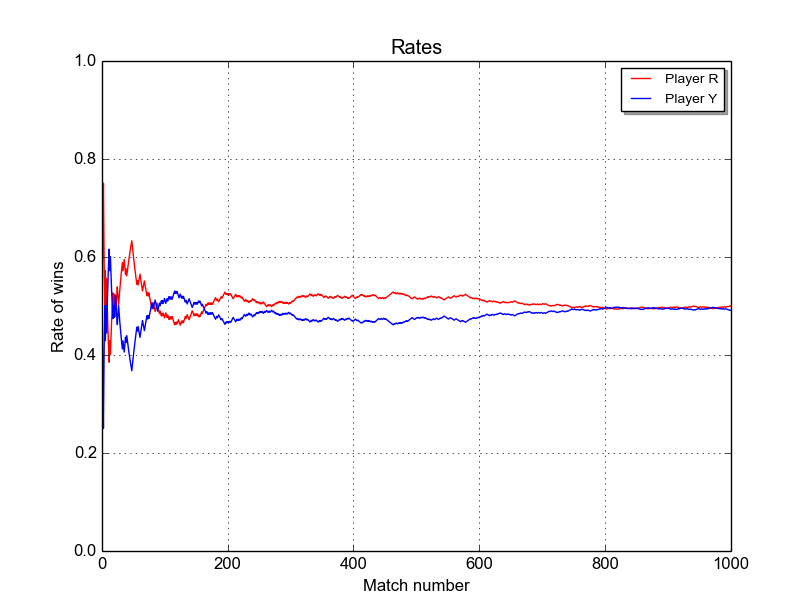
\includegraphics[scale=0.7]{graficos/estabilizacionQLFresh.png}
		\caption{}
	\end{figure}
	

Finalmente llegamos a la conclusión de que la cantidad de iteraciones que necesita nuestro algoritmo para a jugar con cierta superioridad contra un tipo de jugador específico está en el orden de las 1000.

\item ¿Es posible aprender a jugar contra varios tipos de jugadores?

Para este experimento contamos con tres jugadores. La idea fue implementar un regimen de entrenamiento distinto a los que veníamos aplicando. En lugar de entrenar contra un solo adversario, entrenamos por rondas alternadas siguiendo un estilo Round Robin, pero escogiendo al rival al azar en cada ronda. 

$R$ e $Y$ son de tipo bot, en tanto $X$ es de tipo random. Cada ronda dura 12000 iteraciones. Notamos que el jugador $Y$ solo puede aprender cuando le toca jugar con el jugador $R$. En el cuadro \ref{tab:4}
podemos observar que las tasas de victoria parciales son muy similares a las obtenidas por los algoritmos al jugar contra cada tipo de jugador por separado. Esto apoya la conclusión del experimento inmediato anterior.

	\begin{table}[H]
    \centering
	\begin{tabular}{c c c}
      Iteraciones & Jugador & Rate\\
			12000 & X & 0.66425\\
24000 & X & 0.736416\\
36000 & X & 0.751583\\
48000 & X & 0.748583\\
60000 & Y & 0.498583\\
72000 & Y & 0.495583\\
84000 & Y & 0.502416\\ 
96000 & Y & 0.493833\\
108000 & X & 0.751416\\
120000 & Y & 0.510583\\
132000 & X & 0.754833\\
144000 & Y & 0.492333\\
156000 & Y & 0.49375\\
168000 & Y & 0.496333\\
180000 & Y & 0.483833\\
192000 & X & 0.761083\\
204000 & X & 0.761166\\
216000 & Y & 0.502\\
	\end{tabular}
	\caption{Resultados experimento de aprendizaje tipo round-robin}
    \label{tab:4}
	\end{table}


\end{itemize}
\section{Conclusiones y trabajo a futuro}
Quedó en el tintero en esta entrega poder ver el desempeño del agente, entrenado bajo los distintos regímenes, contra un jugador humano. Esto es particularmente importante, pues sería el fin último de este trabajo, conseguir que el agente juegue al nivel de un humano experto. 

Además,  permitiría probar algunas cosas que pueden perderse en los números presentados en este trabajo: si el agente puede bloquear una jugada ganadora del oponente ¿con qué frecuencia lo hace? ¿Cuánto tarda el jugador bot en ganar si no se interfiere con sus jugadas?

Así mismo, vimos en esta entrega que puede no resultar óptimo entrenar al bot solo contra un jugador random. Si bien el regimen de entrenamiento al estilo Round Robin que se intentó no dio resultados particularmente satisfactorios, es un camino interesante para explorar. Plantear nuevos tipos de oponentes (diversificando más los que tenemos) y variar la granularidad de las rondas, pueden ser la diferencia entre un resultado exitoso o no.

\end{document}